%%%
%% Testing :: Functional Testing
%%%
\section{Functional Testing}
\label{sec:functional_testing}

%%%
%% Testing :: Functional Testing :: Usability Requirements
%%%
\subsection{Usability Requirements}
\label{sub:test_func_usability}

\newgeometry{margin=2.5cm}
\begin{landscape}
  \centering
  \setlength\LTleft{0pt}            % default: \parindent
  \setlength\LTright{0pt}           % default: \fill
  \LTcapwidth=\textwidth
  \begin{longtable}{|L{5cm}|L{15cm}|C{2cm}|}
    \hline
    {\bfseries Requirement} & {\bfseries Evidence/Comment} & {\bfseries Outcome} \\
    \hline
    Provide a text field for the user to input the cryptic clue to be solved
    &  A text field has been added to the interface to allow the user to enter a cryptic clue. 
 
\includegraphics[keepaspectratio=true,scale=0.9]{evidence/enterclue.png}
    & PASS \\ \hline
    Provide a drop-down box allowing the user to input the
number of words in the solution, with an initial upper-
limit of 10 words
    & 
\includegraphics[keepaspectratio=true]{evidence/dropdown1.png}

\includegraphics[keepaspectratio=true]{evidence/dropdown2.png}

\includegraphics[keepaspectratio=true]{evidence/dropdown3.png} & FAIL \\ \hline
Dynamically provide individual text boxes for each word
of the solution, which allow the length of the words to be
specified. Also provide check-boxes between these text-
boxes to define whether they are separated by a space
or a hyphen
    & Picture & FAIL \\ \hline
Dynamically provide text boxes to represent each char-
acter of each word of the solution, allowing the user to
input any known characters
    & Picture & FAIL \\ \hline
Provide a table of results which allow the user the to
view the possible solutions
    & A clever rhyme or subtle teaser I constitute & FAIL \\ \hline
Alert the user to required fields with red asterisks
    & A design decision was made to change the colour of the label text 
and the outline of the text box if the user clicks `Submit' without filling in
 required fields.
If the user submits without filling in either required fields:

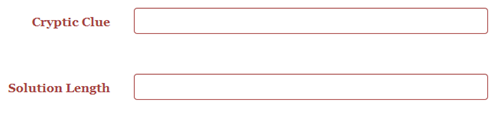
\includegraphics[keepaspectratio=true]{evidence/alert1.png}
If the user submits without filling in the length of the solution: 

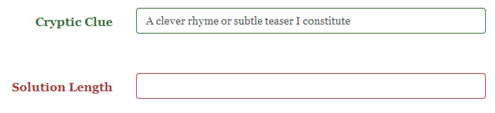
\includegraphics[keepaspectratio=true]{evidence/alert2.png}
If the user submits without filling in the clue field:

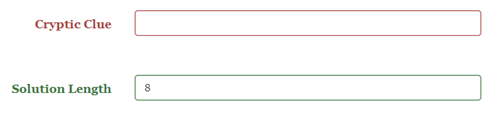
\includegraphics[keepaspectratio=true]{evidence/alert3.png}
 & PASS \\ \hline
Have a consistent layout avoid unnecessary scrolling
    & Picture & FAIL \\ \hline
Alert the user to invalid input through validation checks
with error messages
    & Picture & FAIL \\ \hline
Provide a confidence rating in the table of possible so-
lutions
    & Picture & FAIL \\ \hline
Allow the user to select a proposed solution in the cor-
responding table and mark this as correct
    & Picture & FAIL \\ \hline
Display help buttons to indicate to the user the purpose
and use of each control
    & Picture & FAIL \\ \hline
Provide a button to submit the user input to the appli-
cation for processing
    & Picture & FAIL \\ \hline
Provide a group of radio buttons for the user to select
the clue's orientation in its containing crossword
    & Picture & FAIL \\ \hline
Provide a text box to input the clue's number within its
containing crossword
    & Picture & FAIL \\ \hline
Provide mechanisms to accommodate for users with dif-
ficulties, such as colour-blindness or poor eyesight
    & Picture & FAIL \\ \hline
  \end{longtable}
\end{landscape}